\section{Artificial Neural Network Overview}
This section will give a short overview of the applied network structure and the learning algorithm used for training of the network. The overview will be based on the more detailed explanation in Section~\ref{sec:annSection}.

\subsection{Structure}
Feed-forward will be the preferred architecture for predicting the electricity prices and wind power productions in this thesis. It is the most common structure and data flows from the input to the output layer through the hidden layers in between. The input layer will consist of all the the influential factors of wind power or electricity price and the output will be the predicted price or wind power. Figure~\ref{fig:overviewAnn} illustrates the concept well.

\subsection{Learning}
Training of the network network will be done with the \fnurl{Resilient Back-propagation algorithm}{http://en.wikipedia.org/wiki/Rprop} which is faster than standard Backpropagation \cite{15} and is often used with the \fnurl{feedforward architecture}{http://en.wikipedia.org/wiki/Backpropagation} which we use here \cite{17}. The most significant reason for applying RPROP instead of traditional Backpropagation is its performance and the ability to avoid local minima.

\begin{figure}[h]
\centering
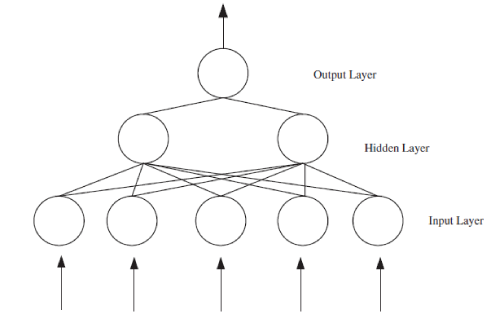
\includegraphics[width=0.8\linewidth]{billeder/ANN.png}
\caption{A simple neural network with 3 layers. \cite{stockForecasting}}
\label{fig:overviewAnn}
\end{figure}

\subsection{Framework}
The framework we will use to conduct our experiments on are \fnurl{Encog Machine Learning Framework}{http://www.heatonresearch.com/encog}. The framework implements the most common Artificial Neural Network structures along with a plethora of learning algorithms. Furthermore, the Resiliet Backpropagation algorithm has been optimized to use multiple processors to perform its tasks which makes it very fast. The framework is implemented in Java and has extensive documentation. The speed was the main reason why we chose this framework.